% This file was created by tikzplotlib v0.9.8.
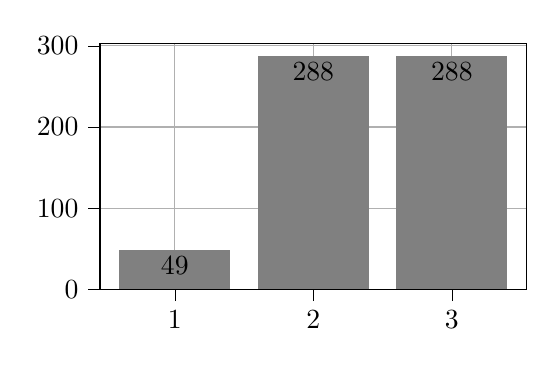
\begin{tikzpicture}

\begin{axis}[
tick align=outside,
tick pos=left,
%title={Dist. between classes},
x grid style={white!69.0196078431373!black},
xmajorgrids,
xmin=-0.54, xmax=2.54,
xtick style={color=black},
xtick={0, 1, 2},
xticklabels = {1,2,3},
y grid style={white!69.0196078431373!black},
ymajorgrids,
ymin=0, ymax=302.4,
ytick style={color=black},
height=4.7cm,
width=7cm,
]
\draw[draw=none,fill=white!50.1960784313725!black] (axis cs:-0.4,0) rectangle (axis cs:0.4,49);
\draw[draw=none,fill=white!50.1960784313725!black] (axis cs:0.6,0) rectangle (axis cs:1.4,288);
\draw[draw=none,fill=white!50.1960784313725!black] (axis cs:1.6,0) rectangle (axis cs:2.4,288);

\node[draw=none,align=center] at (axis cs:0,29) {49};
\node[draw=none,align=center] at (axis cs:1,268) {288};
\node[draw=none,align=center] at (axis cs:2,268) {288};

%\draw (axis cs:0,52) node[
%  scale=0.5,
%  anchor=base west,
%  text=black,
%  rotate=0.0
%]{\bfseries 49};
%\draw (axis cs:1,291) node[
%  scale=0.5,
%  anchor=base west,
%  text=black,
%  rotate=0.0
%]{\bfseries 288};
%\draw (axis cs:2,291) node[
%  scale=0.5,
%  anchor=base west,
%  text=black,
%  rotate=0.0
%]{\bfseries 288};
\end{axis}

\end{tikzpicture}
